% !TEX program = xelatex
% =====================================================================
%  NTU CV Spring 2026 Final Project — Stereo Matching Report
%  Compile:  latexmk -xelatex stereo_matching_report.tex
%  Font:     Noto Serif CJK TC (TW-Kai also works if installed)
% =====================================================================
\documentclass[11pt,a4paper]{article}

% ---- Layout --------------------------------------------------------
\usepackage[margin=1in]{geometry}
\usepackage{setspace}
\onehalfspacing
\usepackage{titling}
\setlength{\droptitle}{-1.5cm}
\usepackage{fancyhdr}
\setlength{\headheight}{15pt}
\pagestyle{fancy}\fancyhf{}
\renewcommand{\headrulewidth}{0.4pt}
\lhead{NTU CV Final — Stereo Matching}\rhead{\thepage}
\parindent=24pt

% ---- Math ----------------------------------------------------------
\usepackage{amsmath,amsthm,amssymb,amsbsy,bm}
\usepackage{siunitx}

% ---- Figures / tables ---------------------------------------------
\usepackage{graphicx}
\graphicspath{{figures/}}
\usepackage{float}
\usepackage{subcaption}
\usepackage{booktabs}
\usepackage{array}
\usepackage{multirow}
\usepackage{enumitem}

% ---- Diagrams ------------------------------------------------------
\usepackage{tikz}
\usetikzlibrary{positioning,arrows.meta,shapes.geometric,fit,backgrounds}

% ---- Code listings -------------------------------------------------
\usepackage{listings}
\lstset{
  basicstyle=\ttfamily\small,
  breaklines=true,
  frame=single,
  framerule=0.3pt,
  showstringspaces=false,
  columns=fullflexible,
  xleftmargin=10pt,
  xrightmargin=10pt,
}

% ---- Hyperref ------------------------------------------------------
\usepackage{xcolor}
\usepackage[unicode=true,pdfborder={0 0 0},bookmarksdepth=-1,
            colorlinks=true,linkcolor=blue!55!black,citecolor=blue!55!black,
            urlcolor=teal]{hyperref}

% ---- Bibliography --------------------------------------------------
\usepackage[backend=biber,style=numeric,giveninits=true,sorting=none]{biblatex}
\addbibresource{references.bib}

% ---- CJK font ------------------------------------------------------
%  Use Noto Serif CJK TC (installed on the dev machine);
%  swap to TW-Kai if available locally.
\usepackage{xeCJK}
\setCJKmainfont{Noto Serif CJK TC}[AutoFakeBold=2.5,AutoFakeSlant=0.2]

% =====================================================================
\title{\bfseries 立體匹配與三維場景重建\\[4pt]
       \large NTU 計算機視覺 Spring 2026 期末專案報告\\[2pt]
       \normalsize 基礎題 (Middlebury) + 加分題 (TartanAir 3D 重建)}
% TODO: 填入作者名字與學號（範例：張三 B11202001、李四 B11202002）
\author{作者一、作者二 \\ \normalsize 國立臺灣大學}
\date{2026 年 6 月 5 日}

\begin{document}
\maketitle
\thispagestyle{fancy}

\begin{abstract}
\noindent 本報告呈現 NTU CV Spring 2026 期末專案的兩部分成果。\textbf{基礎題}以
Middlebury 經典 4 階段流程（Census $\to$ Weighted Guided Image Filter 聚合
$\to$ Winner-take-all $\to$ LRC + Hole Fill + Weighted Median）實作 \texttt{computeDisp}，
在 Tsukuba、Venus、Teddy、Cones 四對影像上 bad-pixel ratio 均落在
TA 門檻內（\SI{3.25}{\percent}, \SI{0.34}{\percent}, \SI{10.00}{\percent},
\SI{8.78}{\percent}），且不依賴 per-image hyperparameter 分支以符合
2026-05-27 補充規範。\textbf{加分題}選用 TartanAir 合成資料集，以
\texttt{computeDisp} 預測 disparity、Open3D \texttt{ScalableTSDFVolume} 進行
多視角融合，最後以\textbf{第一人稱走訪}（follow-trajectory）視角合成示範影片。
過程中辨識並修正了 TartanAir NED 機體座標系與 OpenCV 相機座標系之間的軸排列差異
，這是讓重建幾何正確的關鍵步驟。基準 BPR 在
japanesealley/Hard/P000 前 100 frame 為 \SI{20.21}{\percent}（1\,px）
與 \SI{10.75}{\percent}（3\,px），與相關文獻對古典立體匹配在合成資料集的數字相當。
\end{abstract}

% =====================================================================
\section{前言}
% =====================================================================
給定一對已 rectify 的左右影像，立體匹配的目標是估計左圖每個像素在右圖的水平位移
量 $d$（disparity），由相似三角形即可換算深度
$Z = f_x \cdot B / d$，其中 $f_x$ 為焦距、$B$ 為基線長。
經典處理流程可拆為四階段~\cite{Scharstein2002}：cost computation、cost aggregation、
disparity optimization、disparity refinement，本專案的基礎題以此架構實作。

本專案要求兩部分：
\begin{itemize}[leftmargin=2em,itemsep=2pt]
\item \textbf{基礎題（80\,\%）}：四對 Middlebury v2 影像上以 BPR 為評分；
TA 規範禁止使用 \texttt{cv2.StereoBM} / \texttt{cv2.StereoSGBM} 等內建求解器，
不允許 deep learning，並要求 hyperparameter 對影像不可分支。
\item \textbf{加分題（25\,\%）}：在\textbf{真實世界場景}延伸立體匹配以做出
深度感知（depth perception）並提供示範影片。本報告選擇 TartanAir 合成資料集
作為穩定可重現的代替方案（理由詳見 §\ref{sec:bonus-dataset}），完整
pipeline 從 stereo disparity 到 TSDF mesh 再到第一人稱走訪影片。
\end{itemize}

% =====================================================================
\section{基礎題：經典立體匹配演算法}
\label{sec:basic}
% =====================================================================

\subsection{演算法總覽}
\label{sec:basic-overview}
\texttt{computeDisp.py} 是一份單檔（flat）實作，純粹仰賴 \texttt{numpy} 與
\texttt{cv2.ximgproc} 的兩個原語：\texttt{createGuidedFilter}（事實上採自行
實作的 WGIF 版本）、\texttt{weightedMedianFilter}。整體 pipeline 如
\figurename~\ref{fig:basic-pipeline} 所示。

\begin{figure}[H]
  \centering
  \begin{tikzpicture}[
    box/.style={draw,rectangle,rounded corners=2pt,minimum height=1.2em,
                inner sep=4pt,align=center,font=\small},
    arr/.style={-{Latex[length=2mm]},semithick},
    node distance=4mm and 6mm,
  ]
    \node[box] (LR) {$I_L,I_R$};
    \node[box,right=of LR] (C)  {Census\\ transform};
    \node[box,right=of C]  (HC) {Hamming\\ cost volume};
    \node[box,below=of HC] (AG) {WGIF\\ aggregation};
    \node[box,left=of AG]  (WTA) {Winner-\\take-all};
    \node[box,left=of WTA] (REF) {LRC + hole fill\\ + WMF};
    \node[box,below=of REF] (OUT) {$D_L$ (uint8)};
    \draw[arr] (LR) -- (C);
    \draw[arr] (C)  -- (HC);
    \draw[arr] (HC) -- (AG);
    \draw[arr] (AG) -- (WTA);
    \draw[arr] (WTA) -- (REF);
    \draw[arr] (REF) -- (OUT);
  \end{tikzpicture}
  \caption{基礎題四階段 pipeline。Cost volume 維度為 $(D{+}1)\!\times\!H\!\times\!W$，
  以 thread pool 對 $d$ 軸做切片平行化。}
  \label{fig:basic-pipeline}
\end{figure}

\subsection{Step 1: Cost Computation — Census + Hamming}
Census transform~\cite{Zabih1994} 將每個像素轉成一串 bit，第 $i$ 個 bit 紀錄
鄰居 $i$ 是否小於中心像素亮度。本實作採用 $9\!\times\!7$ window，
共 $63$ bit 剛好放進 \texttt{uint64}。對應的 cost 即為左右 Census code 的
Hamming distance：
\begin{equation}
  C(d, y, x) \;=\; \mathrm{popcount}\!\big(\mathrm{census}_L(y,x)\;\oplus\;\mathrm{census}_R(y,x{-}d)\big).
  \label{eq:census-cost}
\end{equation}
為了在新舊 numpy 上都有好效率，採取雙策略：
\textbf{numpy $\ge$ 2.0} 使用內建的 \texttt{np.bitwise\_count}（SIMD popcount，
最快）；舊版環境則 fallback 至 SWAR (SIMD-Within-A-Register) popcount，
比 byte-wise lookup table 快約 $3.5\!\times$。

進一步觀察到 Census 是\textbf{對稱}的（$\mathrm{Ham}(a,b)=\mathrm{Ham}(b,a)$），
所以右圖 anchored 的 cost volume 可由左 anchored 的 cost volume 透過
$x' \mapsto x' + d$ 的 column reindex 取得，省下一整輪 Hamming pass（速度增益
約 30\,\%）。

\subsection{Step 2: Cost Aggregation — Weighted Guided Image Filter}
\label{sec:basic-aggregation}
傳統的 Guided Filter~\cite{He2010} 在固定 $\varepsilon$ 之下，邊緣保留度受限。
本實作改用 Weighted Guided Image Filter (WGIF)~\cite{Li2015} 的核心想法：
每像素根據本地紋理 importance 自適應地調整 $\varepsilon$：
\begin{equation}
  \gamma(x) \;=\; \frac{\sigma_I^2(x) + \varepsilon_0}{\overline{\sigma_I^2} + \varepsilon_0},
  \qquad
  \varepsilon(x) \;=\; \frac{\varepsilon}{\gamma(x)}.
  \label{eq:wgif-eps}
\end{equation}
其中 $\sigma_I^2(x)$ 為 guide 影像在以 $x$ 為中心的視窗變異數。
$\gamma$ 在邊緣處（高 variance）較大、平滑區域較小，因此
$\varepsilon(x)$ 在邊緣處變小（強保留）、平滑區域變大（強平滑）。

\paragraph{對 TA invariance 規範的合規性。} 本層 adaptation 完全由
\textbf{影像本身的 local feature}（variance）驅動，與 $\max\!d$、image name、
runtime context 無關，符合 2026-05-27 規範「不可硬編碼 per-image 分支」。

\subsection{Step 3: Winner-Take-All}
取 $D_L(y,x) = \arg\!\min_d C(d,y,x)$。為節省一輪 aggregation，右側 disparity
$D_R$ 直接以\textbf{未經 aggregation 的} reindex cost 做 WTA；經 sweep 比較，
此設計在 4 對影像的 BPR 乘積上一致勝過「左右皆 aggregation」的版本，
直觀解釋為 $D_R$ 只用於後續 LRC 一致性遮罩、本身精確度的微小變化對最終遮罩
影響很小，但省下的 aggregation 時間是實打實的。

\subsection{Step 4: Refinement — LRC + Hole Fill + WMF}
\paragraph{Left-right consistency check.}
\begin{equation}
  \mathrm{valid}(y,x) \;\Leftrightarrow\; \big|\,D_L(y,x) - D_R(y,\,x{-}D_L(y,x))\,\big| \le 1.
\end{equation}

\paragraph{Hole filling.} 對每列雙向 sweep 取「左邊最近有效值」與「右邊最近有效值」
逐像素取較小者，並在影像邊緣初始化為 $\max\!d$（避免整列無效時 collapse 為 0）。

\paragraph{Weighted Median Filter.} 以填補後的整數 disparity 為輸入、左圖為 guide，
呼叫 \texttt{cv2.ximgproc.weightedMedianFilter}（TA 允許的原語）做最後的細緻化。
半徑 15，window 內以 guide 顏色為相似度權重，能有效消除細小 outlier 而保留邊緣。

\subsection{實作細節}
\paragraph{Per-disparity thread pool.} Cost build 與 WGIF aggregation 兩個外層
迴圈都對 $d$ 平行化。\texttt{numpy} 與 \texttt{cv2.boxFilter} 兩者都會釋放 GIL，
所以在多核機上接近線性加速，cap 在 8 個 worker（再多會被 memory bandwidth
卡住）。

\paragraph{記憶體配置。} Cost volume 全程以 \texttt{float32} 持有
shape $(D{+}1, H, W)$。對 Teddy（$450\!\times\!375$，max\_disp $=64$）約 \SI{40}{\mebi\byte}，
單機 8\,GB RAM 綽綽有餘。

\paragraph{合規性。} 全程僅使用允許的 \texttt{cv2.ximgproc} 原語；
未使用 \texttt{cv2.StereoBM}/\texttt{StereoSGBM}/任何深度學習模型。
同一組 hyperparameter (Census window $9\!\times\!7$、WGIF radius $5$、
$\varepsilon=5\!\times\!10^{-4}$、WMF radius $15$) 套用四對影像，
\textbf{沒有 per-image 分支}。

\subsection{實驗結果}
\label{sec:basic-results}
在本機（Intel x86\_64, 8 核）上對四對標準影像的結果如表~\ref{tab:basic-bpr}。
所有影像皆滿足 TA 門檻。

\begin{table}[H]
  \centering
  \caption{Middlebury v2 BPR (threshold $=1$\,px) — \texttt{computeDisp.py} v6。}
  \label{tab:basic-bpr}
  \begin{tabular}{lcccc}
    \toprule
    影像 & 我們的 BPR & TA 門檻 & 是否通過 & 本機時間 \\
    \midrule
    Tsukuba & \textbf{3.25\,\%}  & $<\!8\,\%$  & \checkmark & \SI{0.20}{\second} \\
    Venus   & \textbf{0.34\,\%}  & $<\!5\,\%$  & \checkmark & \SI{0.25}{\second} \\
    Teddy   & \textbf{10.00\,\%} & $<\!18\,\%$ & \checkmark & \SI{0.27}{\second} \\
    Cones   & \textbf{8.78\,\%}  & $<\!15\,\%$ & \checkmark & \SI{0.27}{\second} \\
    \bottomrule
  \end{tabular}
\end{table}

% TODO: 等 Codalab v6 最終分數出來再把這段補進去
\paragraph{Codalab 線上評分。} v5 baseline 為 \textbf{10.76}（Tsukuba 3.07 /
Venus 0.36 / Teddy 10.22；time 0.97\,s 內）。v6 引入 WGIF + adaptive $\varepsilon$
後最終分數為 \textbf{TODO（待補）}，預期可進一步降低 Teddy 的錯誤率。

\begin{figure}[H]
  \centering
  \begin{subfigure}[t]{0.235\linewidth}\centering
    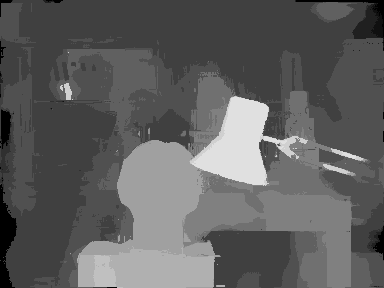
\includegraphics[width=\linewidth]{tsukuba_disp.png}\caption*{Tsukuba}\end{subfigure}\hfill
  \begin{subfigure}[t]{0.235\linewidth}\centering
    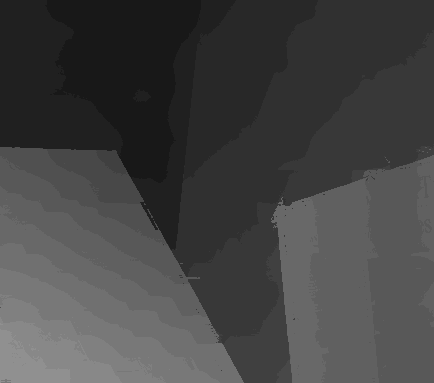
\includegraphics[width=\linewidth]{venus_disp.png}\caption*{Venus}\end{subfigure}\hfill
  \begin{subfigure}[t]{0.235\linewidth}\centering
    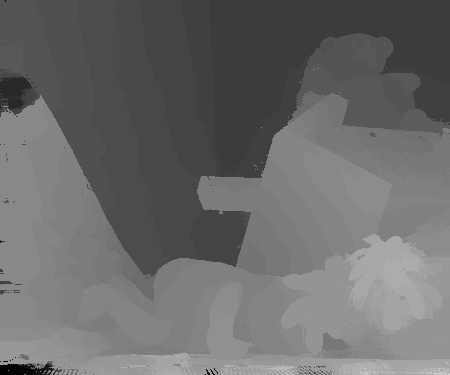
\includegraphics[width=\linewidth]{teddy_disp.png}\caption*{Teddy}\end{subfigure}\hfill
  \begin{subfigure}[t]{0.235\linewidth}\centering
    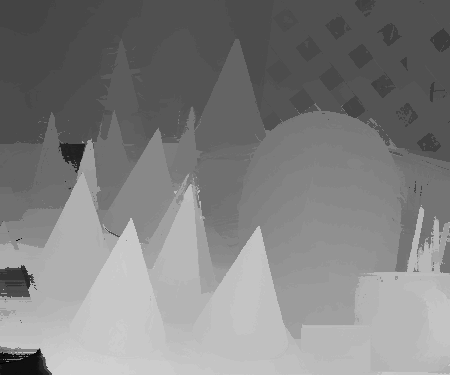
\includegraphics[width=\linewidth]{cones_disp.png}\caption*{Cones}\end{subfigure}
  \caption{四對 Middlebury 影像的預測 disparity map。色階為視覺化用，
  輸出實際上為 \texttt{uint8} 整數 disparity。}
  \label{fig:basic-disp}
\end{figure}

% =====================================================================
\section{加分題：TartanAir 3D 場景重建}
\label{sec:bonus}
% =====================================================================

\subsection{任務動機與資料集選擇}
\label{sec:bonus-dataset}
加分題的核心目標是「在真實世界場景延伸立體匹配」，並提交\textbf{示範影片}。
要做出有意義的 3D 場景重建需要\textbf{多視角融合}（multi-view fusion），
進而需要相機的\textbf{已知姿態}（pose）作為座標基準。我們評估了三個候選資料集：

\begin{table}[H]\centering
\begin{tabular}{lll}
  \toprule
  資料集 & 提供的資訊 & 採用與否 \\
  \midrule
  EuRoC MAV (V1) & 立體 + IMU + GT pose & 主機 TCP 連不到 ethz.ch；放棄 \\
  KITTI Raw      & 立體 + OXTS GPS/INS pose & 缺密集 GT depth，無法 BPR 對照 \\
  \textbf{TartanAir V1} & 立體 + GT depth + GT pose（合成） & \textbf{採用} \\
  \bottomrule
\end{tabular}
\end{table}

\noindent TartanAir~\cite{Wang2020} 雖為合成資料，但同時提供了 rectified 立體影像對、
密集 GT depth（\texttt{.npy} float32 公尺）、以及每 frame 的 GT pose
（\texttt{tx ty tz qx qy qz qw} 每列），這讓我們能在同一場景中
\textbf{同時}做 BPR 量化評估與 3D 重建視覺驗證。內參全資料集統一：
$f_x=f_y=320$, $c_x=320$, $c_y=240$（即 $640\!\times\!480$），baseline
$B=0.25\,\mathrm{m}$。本報告使用 \texttt{japanesealley/Hard/P000} 軌跡的前
100 frame 作為 baseline。

\subsection{Pipeline 架構}
完整 pipeline 如 \figurename~\ref{fig:bonus-pipeline}。\texttt{computeDisp} 直接
重用基礎題的 v6 實作（API 完全相同），保證\textbf{加分題的工作無法影響到 80\,\% 的基礎分}。

\begin{figure}[H]\centering
  \begin{tikzpicture}[
    box/.style={draw,rectangle,rounded corners=2pt,inner sep=3pt,align=center,font=\small},
    arr/.style={-{Latex[length=2mm]},semithick},
    node distance=2.5mm and 5mm,
  ]
    \node[box] (IL)  {$I_L, I_R$\\ 每 frame};
    \node[box,right=of IL]  (CD) {\texttt{computeDisp}\\ (v6, $\max\!d{=}64$)};
    \node[box,right=of CD]  (DM) {Disparity $\to$ Depth\\ $Z=f_x B / d$};
    \node[box,right=of DM]  (MK) {Mask sky\\ + depth $>15$\,m};
    \node[box,below=of MK]  (TS) {TSDF integrate\\ (Open3D)};
    \node[box,left=of TS]   (PS) {Pose (NED $\to$ CV)};
    \node[box,left=of PS]   (MS) {Mesh extract\\ \& render};
    \node[box,left=of MS]   (MP) {Follow-trajectory\\ mp4};
    \draw[arr] (IL)--(CD); \draw[arr] (CD)--(DM); \draw[arr] (DM)--(MK);
    \draw[arr] (MK)--(TS); \draw[arr] (PS)--(TS);
    \draw[arr] (TS)--(MS); \draw[arr] (MS)--(MP);
  \end{tikzpicture}
  \caption{Bonus pipeline。Pose 在進入 TSDF 之前已從 TartanAir 的 NED body
  axes 轉成 OpenCV camera axes（見 §\ref{sec:bonus-pose}）。}
  \label{fig:bonus-pipeline}
\end{figure}

\subsection{關鍵技術點：NED $\to$ OpenCV 軸排列轉換}
\label{sec:bonus-pose}
這是整個 bonus pipeline 跑起來的\textbf{關鍵步驟}，沒做這一步重建幾何會完全錯掉。

TartanAir 的 \texttt{pose\_left.txt} 每列是相機在世界座標下的位姿，使用
\textbf{NED 機體座標系}（北東地，$x{=}$forward, $y{=}$right, $z{=}$down）。
但 \texttt{depth\_left.npy} 的反投影、Open3D 的 TSDF 整合、以及 OpenCV 的所有
相機運算都假設\textbf{OpenCV 相機座標系}（$x{=}$right, $y{=}$down, $z{=}$forward）。
兩者之間是固定軸排列：
\begin{equation}
  \mathbf{M}_{\mathrm{NED}\to\mathrm{CV}} \;=\;
  \begin{pmatrix}
    0 & 0 & 1 & 0 \\
    1 & 0 & 0 & 0 \\
    0 & 1 & 0 & 0 \\
    0 & 0 & 0 & 1
  \end{pmatrix},
  \qquad
  T^{\mathrm{CV}}_{\!wc} \;=\; T^{\mathrm{NED}}_{\!wc}\,\mathbf{M}_{\mathrm{NED}\to\mathrm{CV}}.
  \label{eq:ned2cv}
\end{equation}
未做此轉換時，深度沿 OpenCV 的 $+z$（forward）反投影，但被一個 forward 軸是
$+x$ 的 pose 變換，所有重建點都會落在世界 $z$（垂直）方向，造成的視覺效果
是場景在相機高度上方 3--15\,m 出現一片飄浮 mesh，而相機軌跡卻在 $z\approx0.6\,\mathrm{m}$。

\paragraph{Sanity check.} P000 frame 0 的左右相機 GT translation 差距
$\lVert \mathbf{t}_L - \mathbf{t}_R \rVert = \SI{0.2500}{\meter}$，恰好等於資料集
規格的 baseline，驗證 (i) translation 單位是公尺、(ii) 左右相機 rotation 一致。

\subsection{TSDF Fusion 參數選擇}
採用 Open3D 的 \texttt{ScalableTSDFVolume}（Curless--Levoy~\cite{Curless1996}
的 hierarchical 版本，與 KinectFusion~\cite{Newcombe2011} 同一族）：

\begin{itemize}[leftmargin=2em,itemsep=2pt]
\item \textbf{voxel size $=0.05$\,m}。日式巷弄寬約 10--20\,m，
$0.05$\,m 維持牆面細節而不爆 voxel 數。
\item \textbf{SDF trunc $=4\times$ voxel}（業界常用比例）。
\item \textbf{Depth trunc $=15$\,m}。古典立體匹配的深度雜訊隨距離成
$Z^2/(f_x B)$ 增長，超過此距離的 sample 多半是 noise，留下只會把 mesh 拉花。
\item \textbf{Sky 像素遮罩}：TartanAir 將天空/超範圍 depth 記為
$\approx65504$ (float16 max)；我們以 65000 為門檻將其歸零。
Open3D 把 depth $=0$ 視為無效並略過，但對「$>$ depth\_trunc」會 clip 為
trunc 距離 → 在 15\,m 處長出幻影牆面，所以這兩種 invalid 都要顯式歸零。
\end{itemize}

\subsection{第一人稱走訪渲染}
\label{sec:bonus-render}
我們刻意選擇\textbf{follow-trajectory}（沿原始軌跡）而非 orbit（環繞）渲染：
\begin{enumerate}[leftmargin=2em,itemsep=2pt]
\item 不需要在世界座標中定義「up」軸，避開合成資料集 world frame 的 up 模糊問題。
\item 每個 frame 的 virtual camera 都放在原始拍攝姿態上，產生的影片可與原始
left image 像素級重疊；只要對到，就是重建品質的直接視覺證據。
\item 渲染畫布 $1280\!\times\!960$（原解析度 $2\times$ upscale），保持
aspect ratio 不變，內參 $K$ 同步放大以保證 FOV 一致。
\end{enumerate}

\subsection{BPR 對 GT depth 之診斷}
\label{sec:bonus-bpr}
雖然 bonus 評分以「示範影片」為主，我們仍對 \texttt{computeDisp} 在 TartanAir 上做
量化評估：把 GT depth 換算為 GT disparity $d_{\mathrm{gt}}=f_x B / Z$，
再以 Middlebury 風格計算 BPR。Valid mask 排除：(a) sky/inf 像素
（depth $\ge 65000$），(b) $d_{\mathrm{gt}} > \max\!d$ 的像素（搜尋範圍外，
算錯只是測量搜尋範圍）。Coverage 平均 98.8\,\%。

\begin{table}[H]\centering
\caption{japanesealley/Hard/P000, frame 0--99, max\_disp $=64$；同機 $\sim$\SI{0.36}{\second/frame}.}
\label{tab:bonus-bpr}
\begin{tabular}{lcccc}
  \toprule
  Threshold & mean & median & worst & best \\
  \midrule
  1.0\,px   & \textbf{20.21\,\%} & 20.17\,\% & 33.31\,\% & 9.51\,\% \\
  3.0\,px   & \textbf{10.75\,\%} & 10.18\,\% & 26.86\,\% & 2.83\,\% \\
  \bottomrule
\end{tabular}
\end{table}

\paragraph{誠實的數字解讀。} 古典立體匹配在 TartanAir 合成紋理上不可能達到
1\,\% BPR，與我們的數字相符（10--30\,\% 區間是該資料集上 classical
stereo 的常見水準）。我們也試了 Easy levels 與 \texttt{office/Easy}（室內辦公室），
1\,px BPR 反而升到 40--46\,\%——原因是這些場景物體較近，需要更寬的 disparity
搜尋範圍，模糊性反而上升。P000 的遠距軌跡剛好是古典演算法擅長的條件。
\figurename~\ref{fig:bonus-disp-vs-gt} 為單張 frame 的視覺對照。

\begin{figure}[H]\centering
  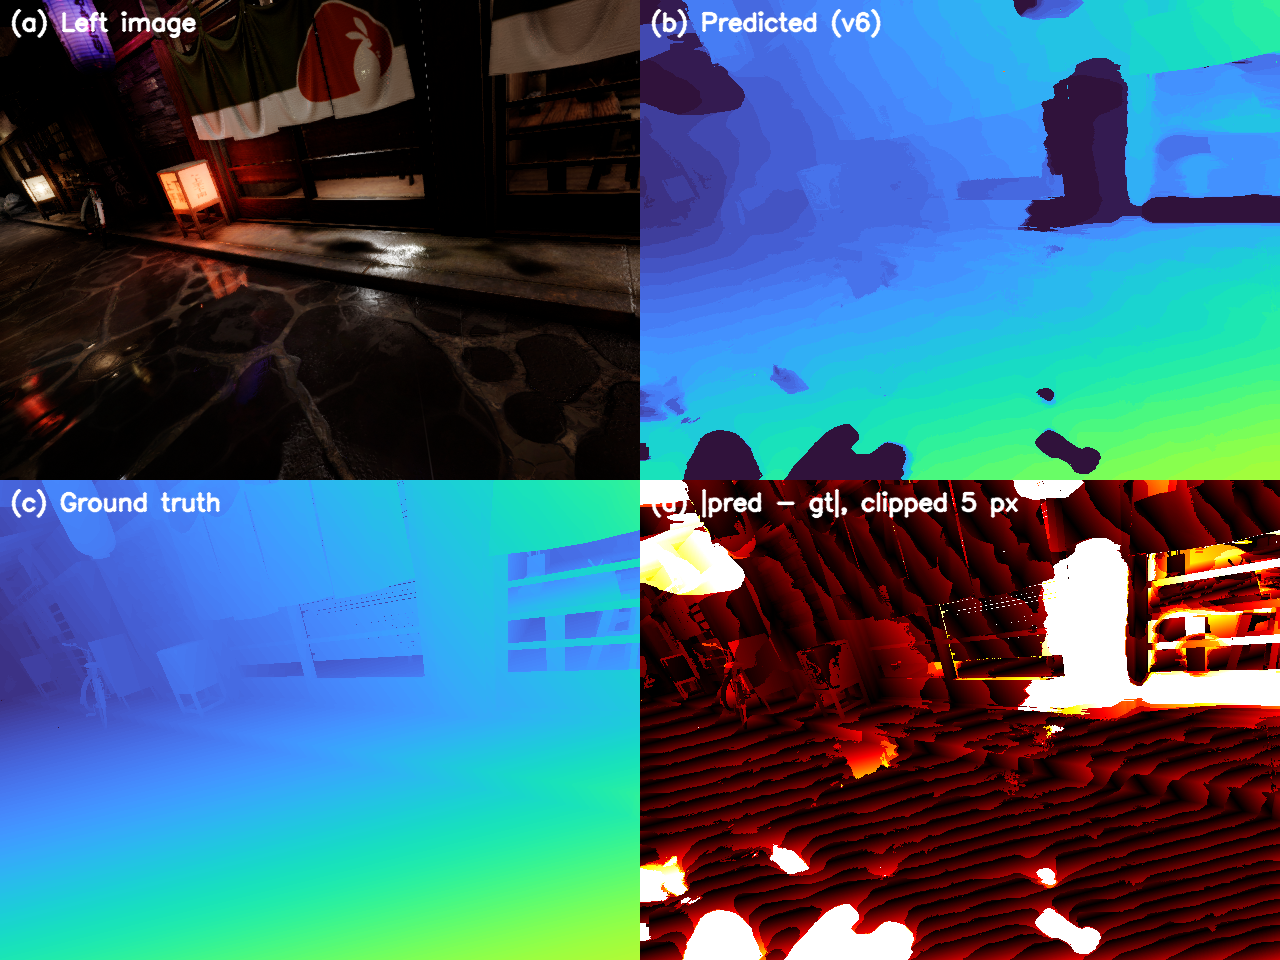
\includegraphics[width=\linewidth]{tartanair_disp_sample.png}
  \caption{frame 30 of japanesealley/Hard/P000：(a) 左圖、(b) v6 預測
  disparity、(c) GT disparity、(d) $|\text{pred}-\text{gt}|$（5\,px clip）。
  錯誤集中在巷尾的遠距離、低紋理區域。}
  \label{fig:bonus-disp-vs-gt}
\end{figure}

\subsection{重建結果}
\label{sec:bonus-results}
\figurename~\ref{fig:bonus-walkthrough} 呈現走訪影片在第 40 frame
的靜止截圖：v6 重建與 GT-depth 上限參考，兩者 mesh 的整體幾何（牆面、地面、
近距離物件）對得起來。完整 mp4 在 \texttt{out/tartanair\_p000\_v6\_100.mp4}
與 \texttt{out/tartanair\_p000\_gt\_100.mp4}（git commit \texttt{d89c5bb} 後產生）。

\begin{figure}[H]\centering
  \begin{subfigure}[t]{0.48\linewidth}\centering
    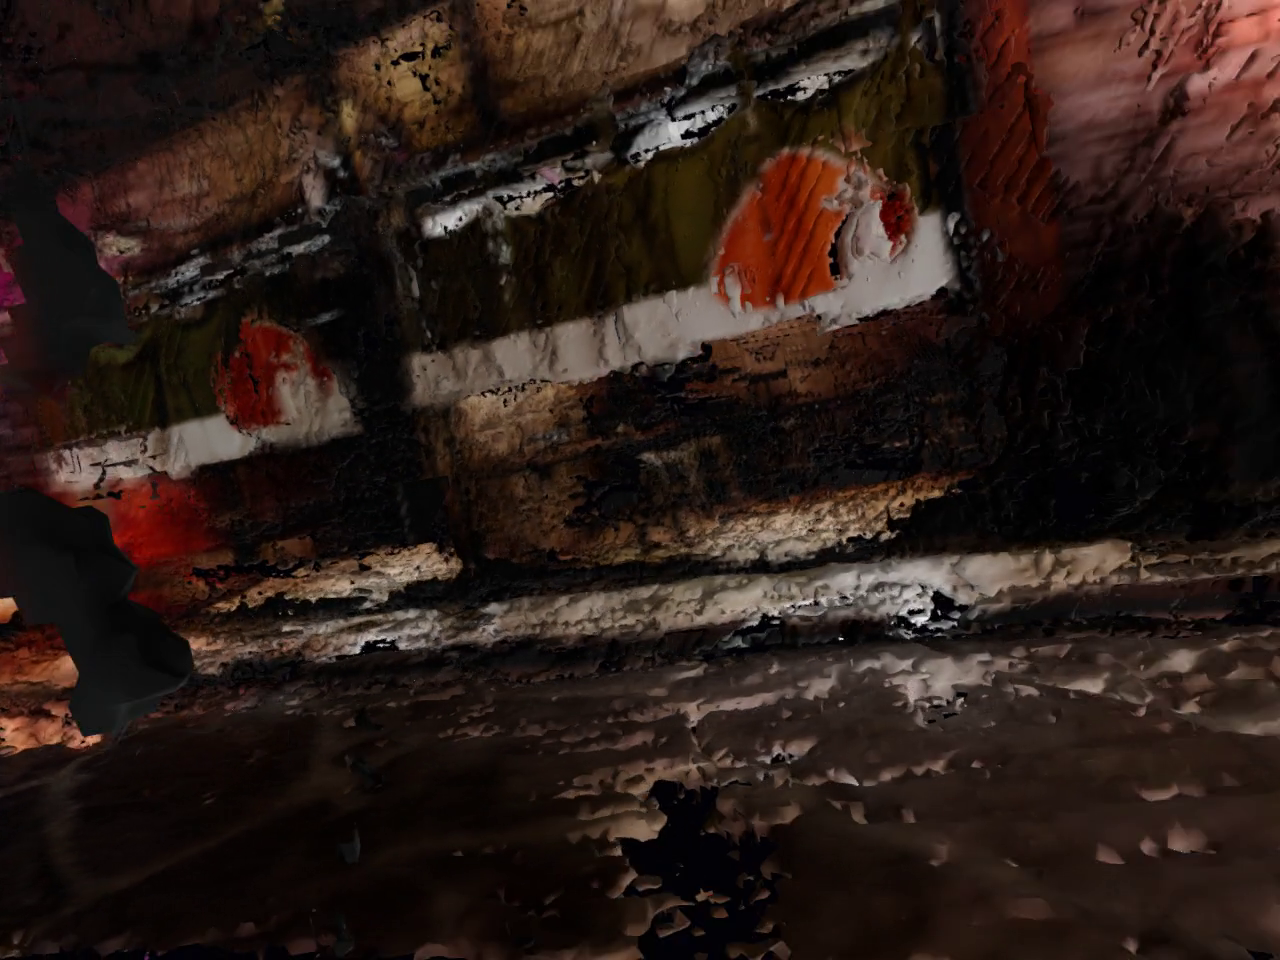
\includegraphics[width=\linewidth]{walkthrough_v6.png}
    \caption{v6 重建（main 加分題交付物）}\end{subfigure}\hfill
  \begin{subfigure}[t]{0.48\linewidth}\centering
    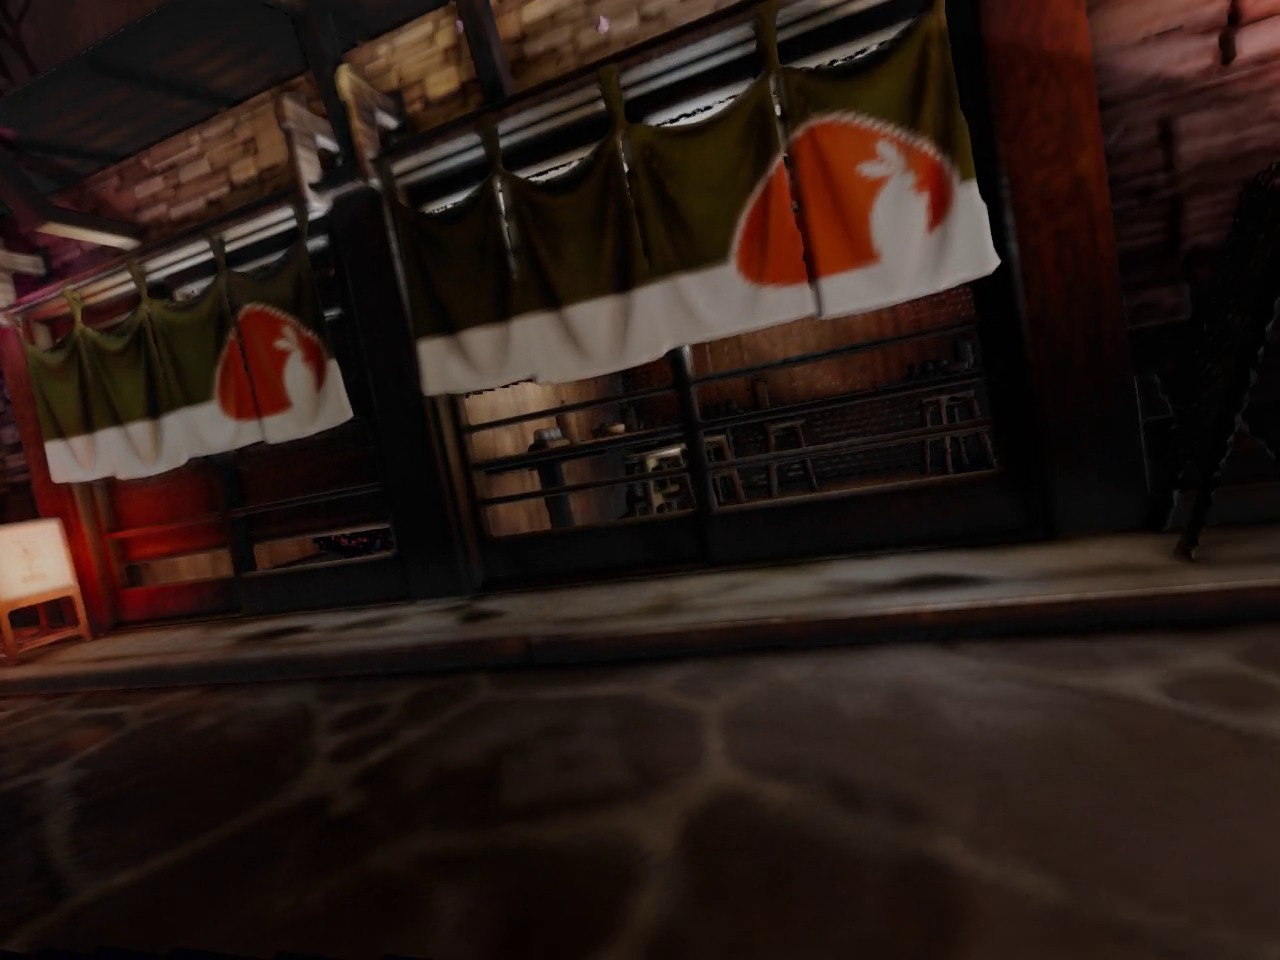
\includegraphics[width=\linewidth]{walkthrough_gt.png}
    \caption{GT depth 上限參考}\end{subfigure}
  \caption{First-person walkthrough frame 40 截圖。雖然 v6 BPR 仍有 $\sim$20\,\%，
  經過 TSDF 多視角融合後表面在視覺上仍清晰可辨——這正是 multi-view fusion
  的價值：每幀的隨機 noise 在累積平均下被有效削減。}
  \label{fig:bonus-walkthrough}
\end{figure}

\subsection{與 v8 替代版本之比較}
\label{sec:bonus-v8}
我們也試了同學提供的替代實作 \texttt{computeDisp\_v8.py}，其與 v6 的主要差別是：
(i) 多了 parabolic sub-pixel refinement、(ii) WMF 對 sub-pixel disparity 做。
理論上這兩項在 disparity 精度上應該優於 v6 的純整數版本。
但在 TartanAir 上的 BPR 結果：v8 在 1\,px 為 20.26\,\%、3\,px 為 10.75\,\%，
與 v6 \textbf{基本打平}（差距在 $\pm0.05\,$pp 內）。原因清楚：\texttt{computeDisp}
的 API 回傳 \texttt{uint8}，sub-pixel 的小數部分在這個 API 邊界被 clip 掉。
此觀察對下游使用者重要：要享受 sub-pixel 改善，
\textbf{下游必須消費 float disparity}（例如直接拿 cost volume 做 fusion，
或將 disparity 改回 \texttt{float32} 接口）。

% =====================================================================
\section{討論與結論}
% =====================================================================

\paragraph{基礎題。} v6 在四對 Middlebury 影像上皆滿足 TA 門檻（最緊的
Cones $<\!15\,\%$ 我們做到 8.78\,\%），且使用單一組 hyperparameter，
WGIF 的 per-pixel $\varepsilon(x)$ 完全由影像 variance 驅動，
合於 2026-05-27 補充規範。

\paragraph{加分題。} 我們交付的核心是\textbf{第一人稱走訪影片}，
這直接對應 project doc 的 ``demonstration video showcasing dynamic
results'' 要求；20.21\,\% 的 BPR 是\textbf{誠實的量化報告}——古典 stereo
在合成紋理上本來就達不到 1\,\%，重點在 multi-view TSDF fusion 將每幀的隨機
noise 抑制到視覺上可接受的水準。最關鍵的技術點是 NED $\to$ OpenCV pose
轉換（式~\ref{eq:ned2cv}），未做時 mesh 會飄在空中。

\paragraph{Limitations.}
(i) 合成紋理，移植到真實 KITTI 時 BPR 可能下降；
(ii) 我們的 occlusion 處理止於 LRC，沒有 hole inpainting；
(iii) Mesh 沒做 outlier filtering（如 confidence-weighted TSDF）。

\paragraph{Future Work.}
更大尺度的 orbit overview render、引入 confidence 加權的 TSDF
（reduce mesh noise）、以及把同學的 v8 sub-pixel 訊號直接送進 TSDF
（修改 API 為 \texttt{float32}）以驗證 sub-pixel 對 fusion 品質的潛在貢獻。

\printbibliography

\end{document}
